
\documentclass[paper=a4, fontsize=11pt]{scrartcl} % A4 paper and 11pt font size

\usepackage[T1]{fontenc} % Use 8-bit encoding that has 256 glyphs
\usepackage{fourier} % Use the Adobe Utopia font for the document - comment this line to return to the LaTeX default
\usepackage[german]{babel} % English language/hyphenation
\usepackage{amsmath,amsfonts,amsthm} % Math packages

\usepackage{lipsum} % Used for inserting dummy 'Lorem ipsum' text into the template

\usepackage{sectsty} % Allows customizing section commands
\allsectionsfont{\centering \normalfont\scshape} % Make all sections centered, the default font and small caps
\usepackage{minted}
\usepackage{graphicx}
\usepackage{fancyhdr} % Custom headers and footers
\pagestyle{fancyplain} % Makes all pages in the document conform to the custom headers and footers
\fancyhead{} % No page header - if you want one, create it in the same way as the footers below
\fancyfoot[L]{} % Empty left footer
\fancyfoot[C]{} % Empty center footer
\fancyfoot[R]{\thepage} % Page numbering for right footer
\renewcommand{\headrulewidth}{0pt} % Remove header underlines
\renewcommand{\footrulewidth}{0pt} % Remove footer underlines
\setlength{\headheight}{13.6pt} % Customize the height of the header

\numberwithin{equation}{section} % Number equations within sections (i.e. 1.1, 1.2, 2.1, 2.2 instead of 1, 2, 3, 4)
\numberwithin{figure}{section} % Number figures within sections (i.e. 1.1, 1.2, 2.1, 2.2 instead of 1, 2, 3, 4)
\numberwithin{table}{section} % Number tables within sections (i.e. 1.1, 1.2, 2.1, 2.2 instead of 1, 2, 3, 4)

%\setlength\parindent{0pt} % Removes all indentation from paragraphs - comment this line for an assignment with lots of text

%----------------------------------------------------------------------------------------
%	TITLE SECTION
%----------------------------------------------------------------------------------------

\newcommand{\horrule}[1]{\rule{\linewidth}{#1}} % Create horizontal rule command with 1 argument of height

\title{	

\includegraphics[width=0.6\linewidth]{img/Mathnatlogo.png}\\[1cm]
\normalfont \normalsize 
\textsc{Master Praktikumsarbeit} \\ [25pt]
\horrule{0.5pt} \\[0.4cm] 
\huge Grenzen der Leistungsfähigkeit und architektonische Beschränkungen der BlueField-3 \\ % The assignment title
\horrule{0.5pt} \\[1.6cm]
}

\author{Sten Heimbrodt} % Your name

\date{\normalsize\today} % Today's date or a custom date
\newpage
\begin{document}

\maketitle % Print the title

\tableofcontents
\newpage
\section{Einleitung}
Das Problem der Lastverteilung stellt eines der fundamentalsten in der Informatik dar. Viele Strategien und Ansätze prägen dabei die Landschaft der Implementierungen und variieren teils stark im jeweiligen Energieverbrauch. Seit geraumer Zeit begegnen Hersteller solchen Problemen mit technischen und architektonischen Lösungen. So entwickelt sich der Trend hin zu einer heterogenen Compute Landschaft. Die hier vorliegende Arbeit beschäftigt sich mit der Klasse der SmartNICs, im speziellen der BlueField-3 von Nvidia. Es werden technische Limitierungen anhand von Experimenten untersucht sowie ein gewisser Anteil an reverse Engineering betrieben, um Licht auf die Architektur zu werfen. Diese wird leider seitens Nvidia als proprietär betrachtet und dementsprechend nicht veröffentlicht. Außerdem wird die Flow API aus dem DOCA Framework verwendet, um die speziellen Hardwarebeschleuniger zu programmieren, die den eigentlichen energetisch Effizienten Vorteil bringen. Diese Arbeit versucht also ebenfalls, ein Verständnis für die API zu schaffen, um auch andere Probleme mittels DOCA Flow implementieren zu können.
\subsection{Ziele dieser Arbeit}
Ziel ist es, die technischen Limitationen, die so nicht im Material seitens des Herstellers genannt werden, zu ermitteln. Außerdem soll mithilfe eines architektonischen Gesamtkonzepts versucht werden, die Menge an Problemen genauer zu beschreiben, die auf SmartNICs sinnvoll ausgeführt werden können und von den Leistungsgewinnen profitieren.
\section{BlueField Architektur}
Zunächst ist die grundlegende Architektur der BlueField‑3 vorzustellen. Bei diesem System handelt es sich um eine Netzwerkkarte der Klasse der SmartNICs. Diese zeichnen sich dadurch aus, dass neben den Komponenten einer konventionellen Netzwerkkarte zusätzliche, herstellerseitig integrierte Hardwarebeschleuniger bereitgestellt werden. Außerdem wird im Falle der BlueField noch ein komplett eigener ARM-Host verbaut, der es ermöglicht, Anwendungen vollständig vom eigentlichen Host, in dem die BlueField verbaut ist, gekapselt auszuführen. Diese Beschleuniger decken unterschiedliche Funktionen ab und sind selbst keine klassischen Prozessoren, sondern entweder Application-Specific Circuits (ASICs) oder Field-Programmable Gate-Arrays (FPGAs). Der Vorteil solcher spezialisierter Hardware ist einerseits die enorm bessere Energieeffizienz und andererseits die daraus resultierenden Geschwindigkeitsgewinne. Dies wird bei SmartNICs besonders offensichtlich, da es sich um eine sehr hochfrequente Verarbeitungspipeline handelt, weil der Nutzer und der Host das Netzwerk als möglichst in Echtzeit wahrnehmen wollen. Daher ist jegliche Verarbeitung von Daten auf Seiten der Netzwerkkarte verpflichtet, sämtliche Operationen derart zu modellieren, dass die Latenz in einem möglichst kleinen Umfang bleibt. Das größte zu minimierende Problem ist bei solchen Operationen, die absolute Anzahl an Taktzyklen möglichst gering zu halten oder sogar im optimalen Fall vollständig zu umgehen. Dabei setzen ASICs und FPGAs vor allem auf ihre großen Datenbusse, die dazu genutzt werden können, das Paket vollständig auf einen Datenpfad zu legen und entsprechend zu verarbeiten. Es wird dazu die Eigenschaft von klassischen Netzwerkpaketen ausgenutzt, dass Pakete meist an erwartbaren Bitpositionen die jeweiligen Informationen codieren. Eine weitere wichtige Unterscheidung, die für die späteren Experimente relevant ist, sind die beiden Datenpfadklassen von \textbf{On-Path} und \textbf{Off-Path}. On-Path bedeutet im wesentlichen, dass alle zugehörigen Beschleuniger und Komponenten gezwungenermaßen immer an der Verarbeitung beteiligt sind. Dabei ist natürlich auch klar, dass bei fehlender Performance sofort ein Flaschenhals entsteht, der die allgemeine Datenrate direkt beeinflusst. Off-Path-Komponenten hingegen können bei Bedarf in den kritischen Datenpfad integriert werden, um beispielsweise zusätzliche Funktionalität zu gewährleisten, wie das Parsen von bestimmten anderen Bitpositionen innerhalb des Pakets. Der besagte On-Path, also der kritische Datenpfad, ist in Abbildung 2.1 auf der rechten Seite über den Netzwerk Ein- und -Ausgang zu erkennen. Die entsprechenden Off-Path-Komponenten sind auf der linken Seite zu sehen und sind mittels PCIe Switch mit dem entsprechenden ARM-Host verbunden.
\begin{figure}
    \centering
    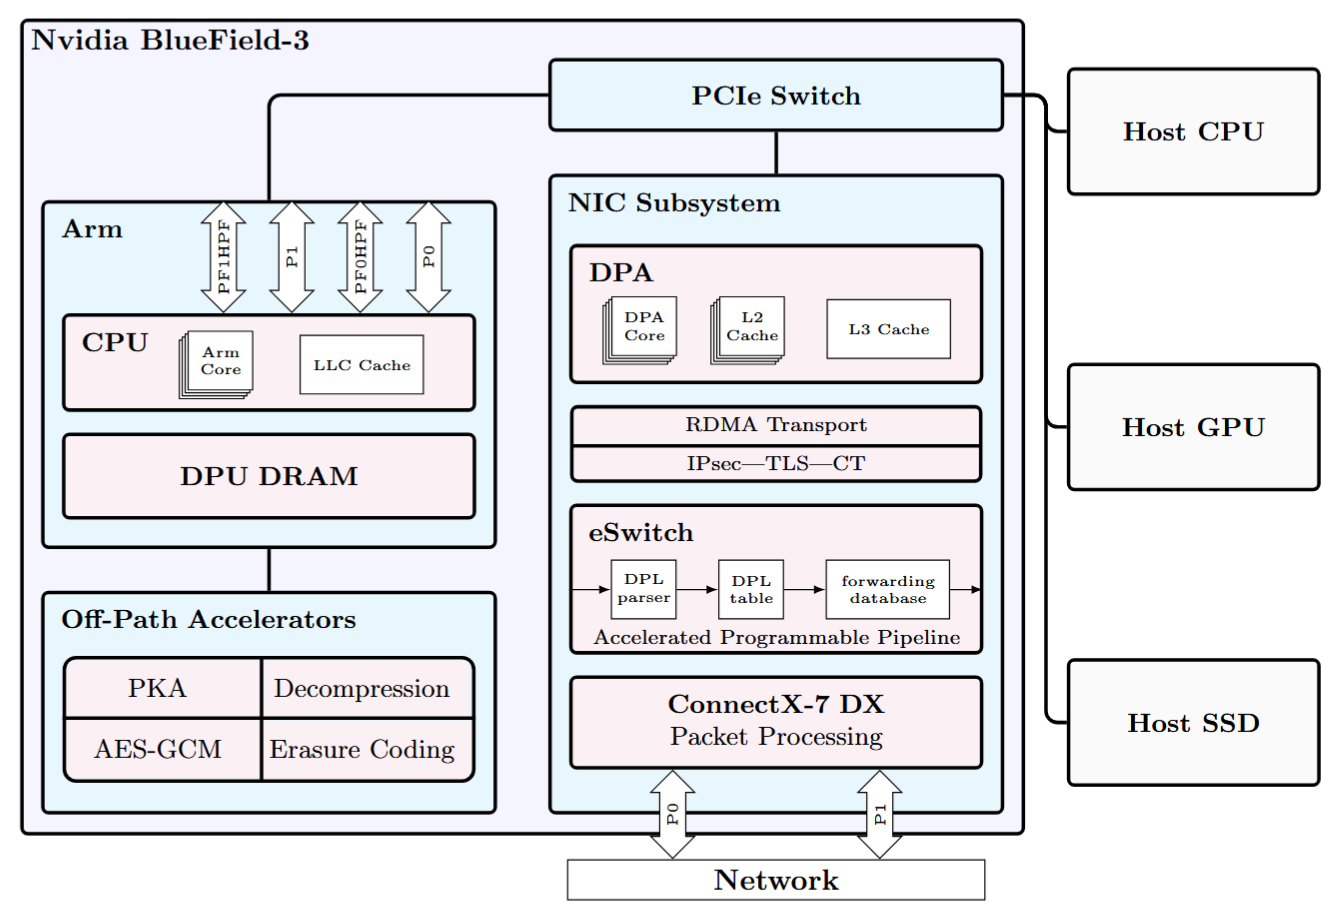
\includegraphics[width=1\linewidth]{img/bluefield.png}
    \caption{BlueField-3 Architektur}
    \label{fig:placeholder}
\end{figure}
\subsection{DOCA Flow}
Nvidia gibt der Kundschaft mit DOCA ein sehr mächtiges Werkzeug an die Hand, um selbst Anwendungen für die BlueField- sowie die ConnectX-Plattform zu entwickeln. Dabei bildet DOCA selbst einen Überbegriff für eine Menge von speziellen Bibliotheken, welche alle meist ein oder mehrere Funktionen eines Hardwarebeschleunigers abdecken. Für diese Projektarbeit ist das sogenannte \textbf{DOCA Flow} Framework verwendet worden. Es erlaubt die direkte Programmierung des \textbf{eSwitch} , welcher, wie in Abbildung 2.1 zu sehen, die erste und in speziellen Fällen auch einzige ausgeführte Hardwareeinheit ist. DOCA Flow kann aus den üblichen Paketquellen des jeweiligen Linux Betriebssystems installiert werden und besteht aus offenen und teils kommentierten C-Header-Files und vorkompilierten Shared-Object-Bibliotheken. Nvidia bietet außerdem eine Dokumentation sowie eine Reihe von Beispielen an, die entsprechend der Problemstellung als Implementierung vorliegen. Diese \textbf{Samples} werden ebenfalls mit DOCA Flow mitinstalliert.
\subsubsection{Pipes und Entries}
\begin{figure}
    \centering
    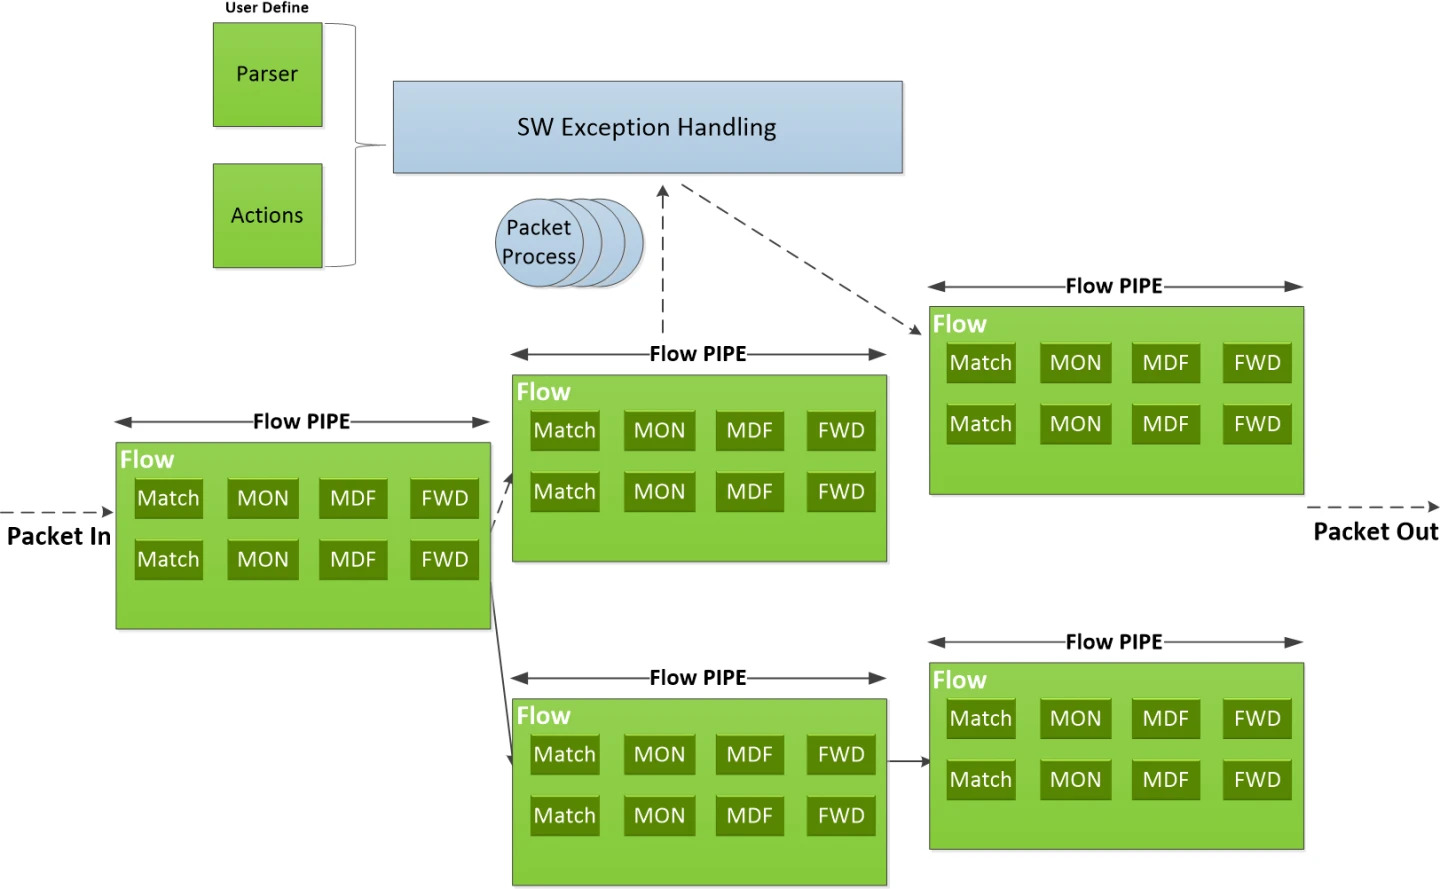
\includegraphics[width=1\linewidth]{img/docscontent.nvidia.jpg}
    \caption{Pipe Verschachtelung}
    \label{fig:placeholder}
\end{figure}
Die zwei grundlegendsten Konzepte von DOCA Flows sind die der sogenannten \textbf{Pipes} und \textbf{Entries}. Diese beiden bilden zusammen den Kern der Funktionalität von DOCA Flow und erlauben neben den interessanten Paketmodifikationen (\textit{Actions}) auch weitere Features wie beispielsweise \textit{Matching}, \textit{Monitoring} und \textit{Forwarding}. Matching definiert zunächst anhand einer genauen Bitfelddefinition, welche Pakete explizit oder implizit aus dem Datenverkehr der Netzwerkkarte herausgenommen werden sollen und im weiteren Verlauf verarbeitet werden können. Das Monitoring erlaubt uns hierbei, ohne weiteren Overhead die Menge sowie die Größe des entsprechenden Netzwerkverkehrs zur Laufzeit beobachten zu können. Daraufhin werden die eigentlichen Actions ausgeführt, die es nun erlauben, Bitfelder auf L2, L3 und L4 des Pakets zu ändern. Abschließend wird mittels der Forwardingdefinition angegeben, an welches Ziel das verarbeitete Paket final weitergeleitet werden soll. Als Ziel können neben dem Hardware-Port auch Pipes oder sogar der ARM-Host angegeben werden. Die genannten Komponenten befinden sich allgemein in einer Pipe. Diese stellt eine Art Template dar, mit dem dann in den Entries die eigentlichen Implementierungen der genannten vier Bereiche zu finden sind. Entries werden einer entsprechenden Pipe zugeordnet und können nur solche Bitfelder beeinflussen, die als Template innerhalb der Pipe aktiviert wurden. Durch das Verketten von Pipes können hochkomplexe Anwendungen implementiert werden (siehe Abbildung 2.2).

\subsubsection{Hash-Pipes}
Hash-Pipes stellen einen besonderen Typ von Pipe dar. Sie erlauben die implizite Ausführung eines Hashing Algorithmus auf eingehende Pakete. Dieser Hashing Algorithmus erlaubt es dann, entsprechend des Ergebnisses der Anwendung einer Hashing Funktion Pakete auf der Pipe zugeordneten Entries zu verteilen. Dabei ist es nicht möglich, den entsprechenden Hashing-Algorithmus zu bestimmen, sondern es wird lediglich eine implementierung seitens Nvidia angeboten. Allerdings lassen sich gewisse Parameter anpassen, die es beispielsweise erlauben, alle Pakete an alle Entries zu senden oder die gewählten Bitfelder, die in den Hashing Algorithmus einfließen sollen, zu ignorieren und alle Pakete vollständig zufällig an alle Entries zu verteilen. Über welche Bitfelder gehashed werden soll, wird mittels der match Maske definiert. So kann beispielsweise entschieden werden, nur über den Source-Port zu hashen. 
\subsection{Hardware Beschleuniger}
%hier auf eSwitch, DPL-Parser, DPL-MatchAction eingehen
Der für diese Arbeit wohl wichtigste Hardware-Beschleuniger ist der vorher genannte eSwitch. Dieser setzt sich im wesentlichen aus drei Komponenten zusammen. Grundsätzlich wird der eSwitch mithilfe einer P4-abgewandelten Sprache namens DOCA Pipelining Language (DPL) programmiert. Die DPL wiederum beschreibt das Verhalten der drei Hauptbestandteile des eSwitches. Zunächst einmal treffen Pakete beim \textbf{DPL-Parser} ein. Dieser bricht das zunächst serielle Paket in eine Bitfeld Repräsentation auf und ermöglicht so die schnellen und Effizienten Bitwise Operationen innerhalb der ASICs. Daraufhin werden die Pakete an die \textbf{DPL-table} weitergeleitet. Diese enthält die Kombination eines Matches und einer entsprechenden Action und ist somit die Kernausführungs-Einheit im eSwitch. Schlussendlich werden die Pakete entsprechend der Einträge in der \textbf{Forwarding-Datenbank} an das entsprechende Ziel weitergeleitet. Der Zusammenhang dieser drei Einheiten ist ebenfalls in Abbildung 2.1 zu sehen. \newpage
\section{XenoFlow 0.1}
\textit{Dieses Projekt ist als Anschluss an die Ursprüngliche Implementierung eines Loadbalancers zu verstehen, den ich im Rahmen meiner Bachelorarbeit im ersten Quartal 2025 implementiert habe. Zum damaligen Zeitpunkt war es aufgrund des Umfangs der Thematik nicht möglich, auf architektonische Details einzugehen, was allerdings nun in diesem Rahmen passieren soll.}
\subsection{Was bisher geschah...}
\begin{figure}
    \centering
    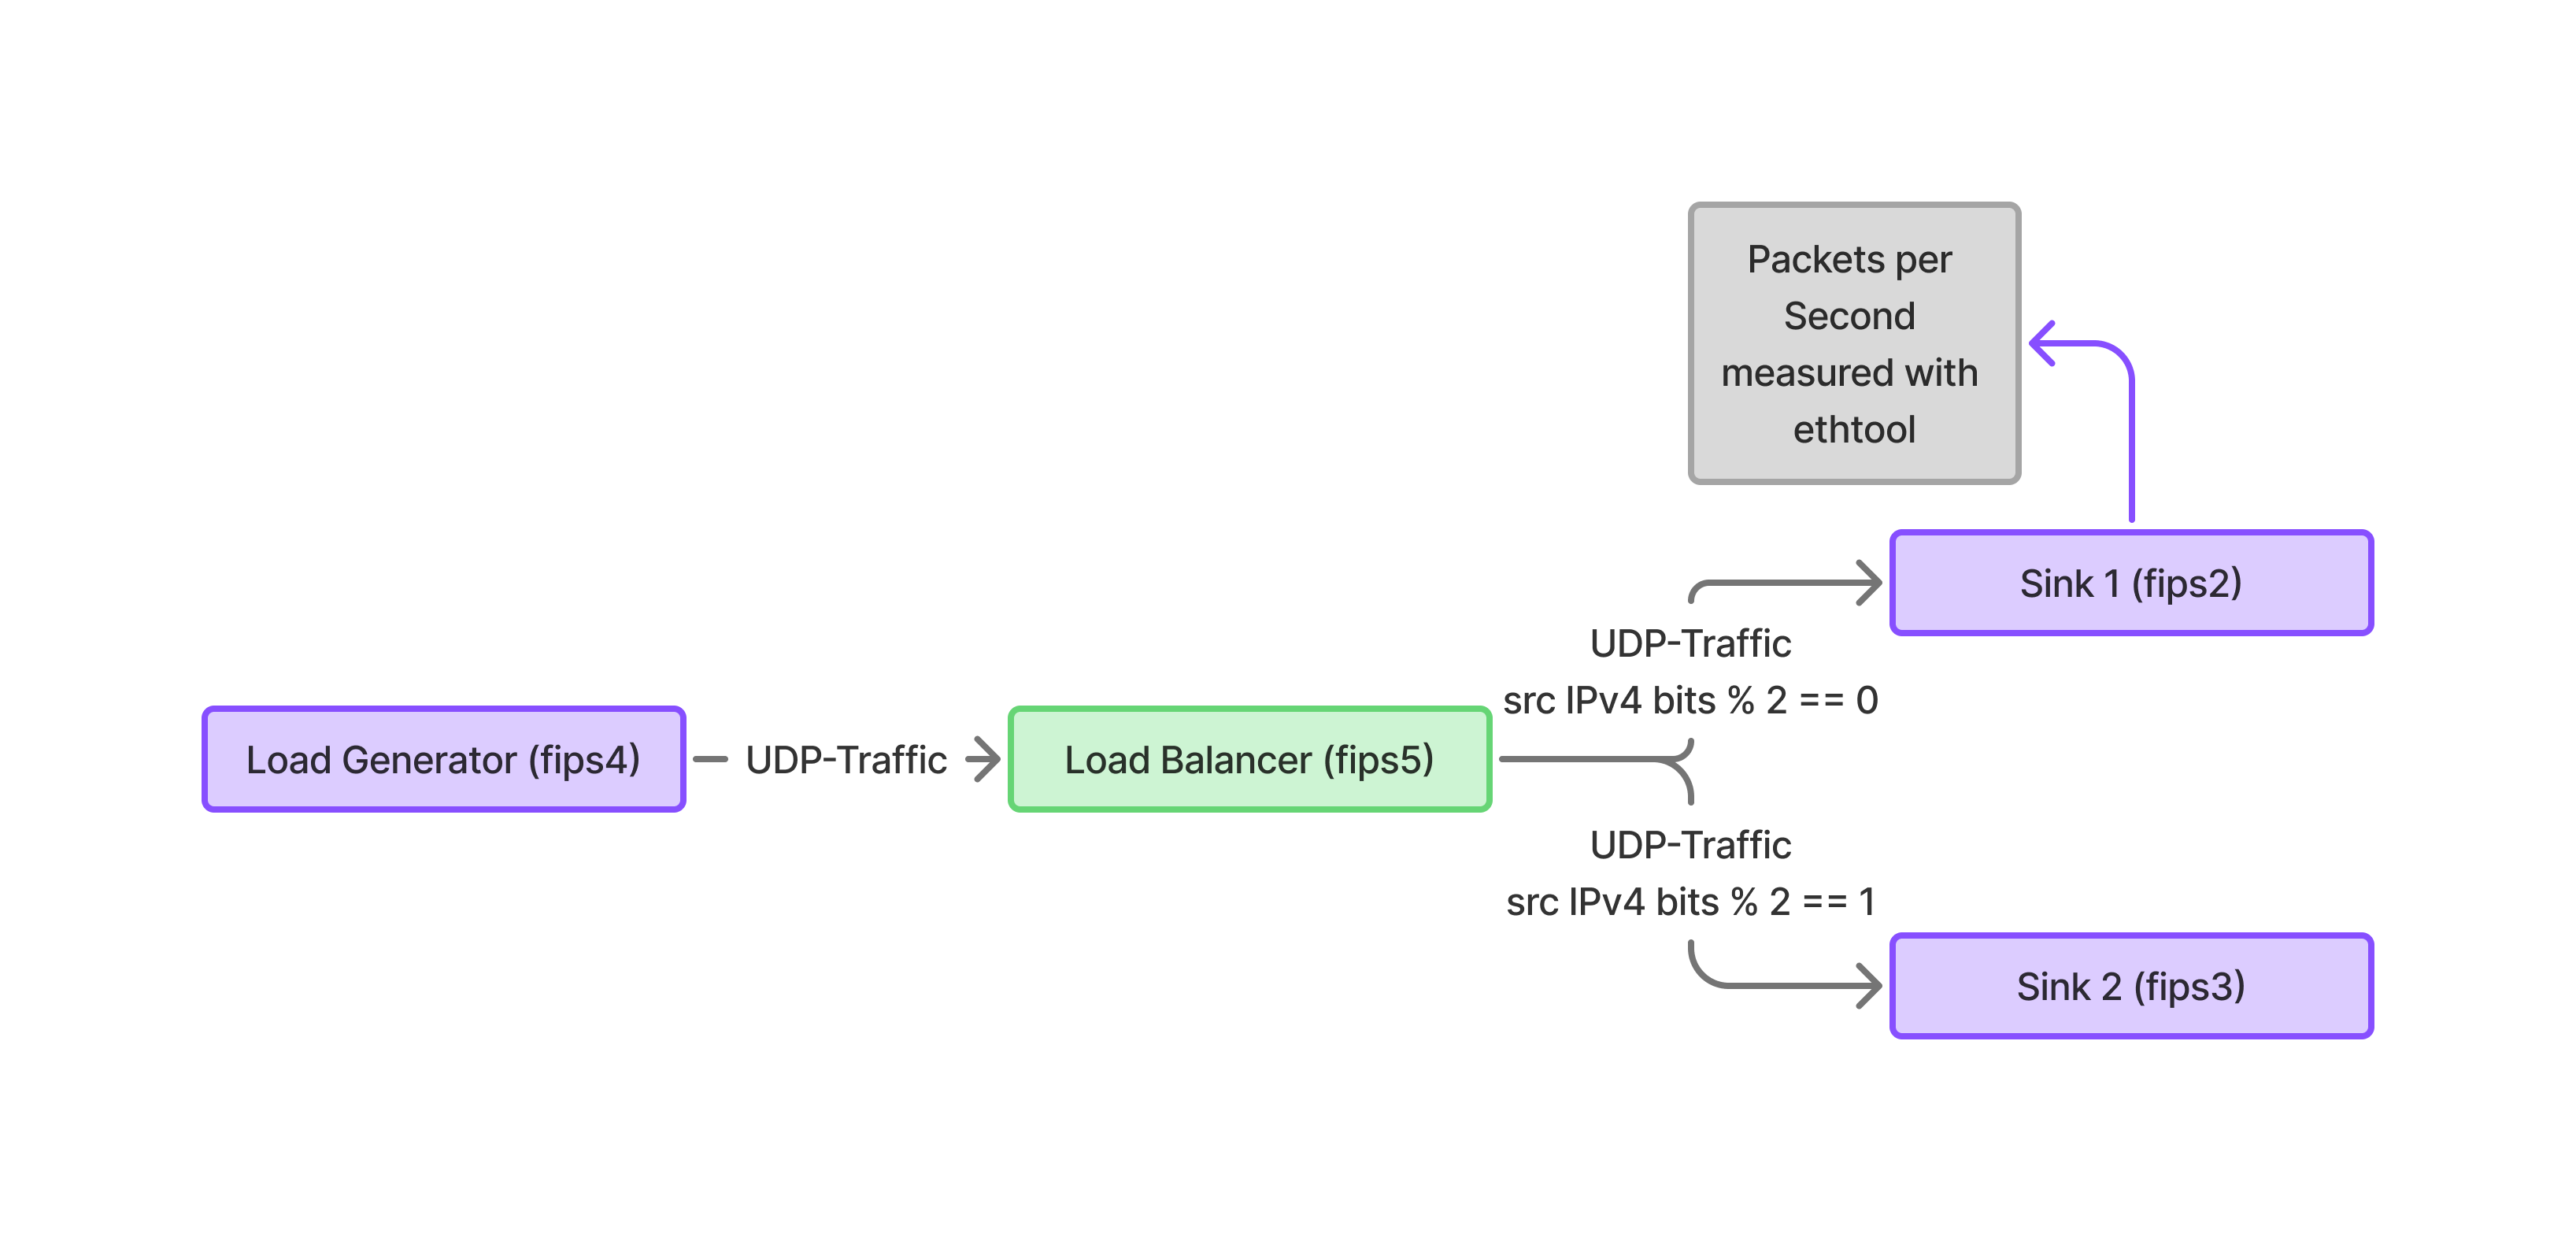
\includegraphics[width=1\linewidth]{img/Messaufbau PPS.png}
    \caption{Prototyp XenoFlow mit zwei Backends}
    \label{fig:placeholder}
\end{figure}
XenoFlow war in seiner ursprünglichen 0.1 Fassung ein L3-Loadbalancer, der anhand der Source-IP-Adresse mithilfe eines selbst implementierten, bitfeldbasierten Pseudohashings die Lastverteilungsentscheidung getroffen hat. Dabei wurden je nach Anzahl der aktiven ansprechbaren Backends die letzten Bits der Source-IP-Adresse als Matchkriterium für die Entries verwendet, die daraufhin schließlich an das entsprechende Backend mittels eines Des-tination-MAC-Adressen-Rewrites weitergeleitet wurden. Das gesamte Projekt wurde damals mittels DOCA Flow implementiert. Grundsätzlich war der Loadbalancer allerdings sehr statisch. Es wurde zu Programmstart einmal aus einer Config-YAML-Datei die aktuelle Konfiguration ausgelesen und entsprechend installiert. Es war also besonders keine Änderung der Backends zur Laufzeit möglich. Außerdem hatte der pseudo Hashingalgorithmus das Problem, dass er anfällig für Struktur in IP-Adressen war, da ein Filtern keiner direkten Hashfunktion entspricht. Es musste also davon ausgegangen werden, dass die letzten Bits der Source-IP-Adresse ausreichend hoch entropisch sind, um äquivalent große Klassen von Paketen für die Lastverteilung zu erzeugen. Diese Funktionsweise ist in Abbildung 3.1 dargestellt.
\subsection{Ergebnisse}
\begin{figure}
    \centering
    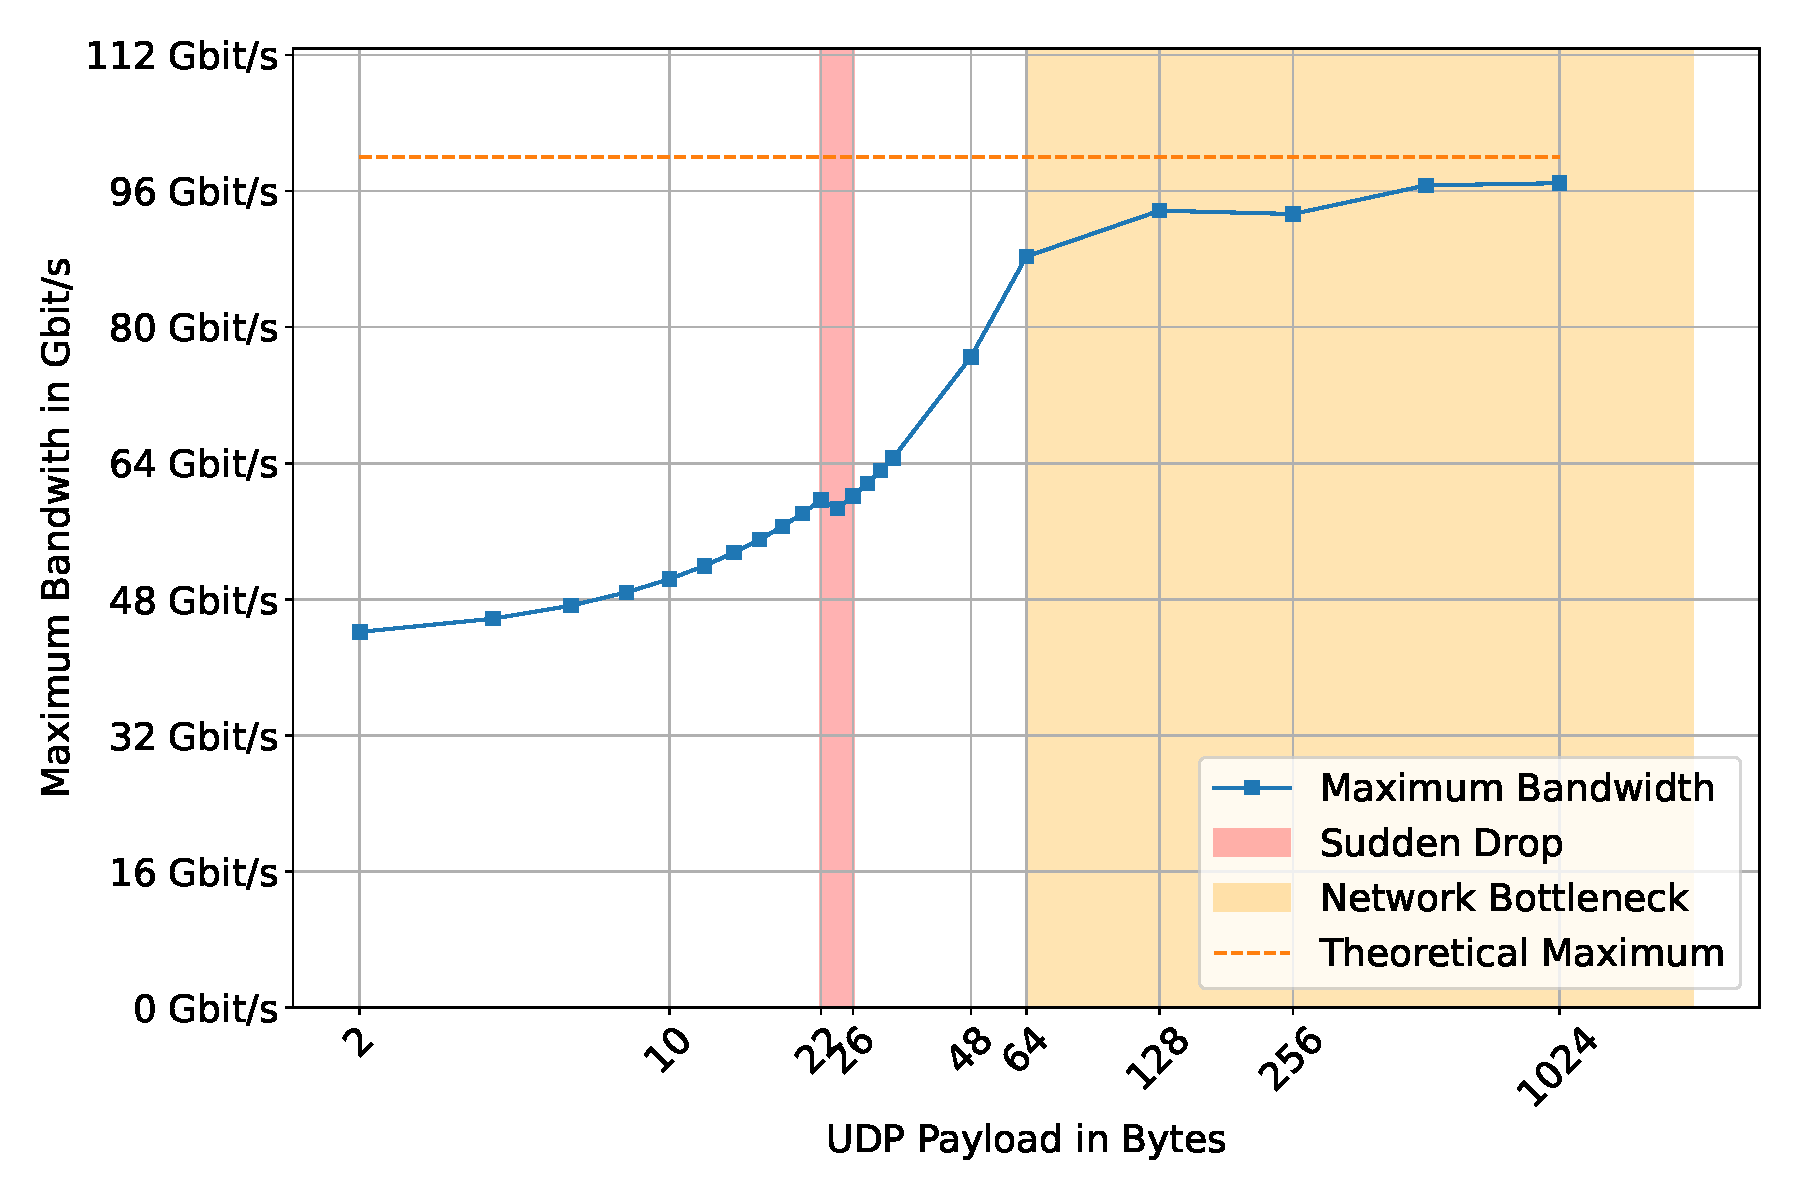
\includegraphics[width=1\linewidth]{img/pps_bandwidth.pdf}
    \caption{Pakete pro Sekunde - Bandbreite}
    \label{fig:placeholder}
\end{figure}
\begin{figure}
    \centering
    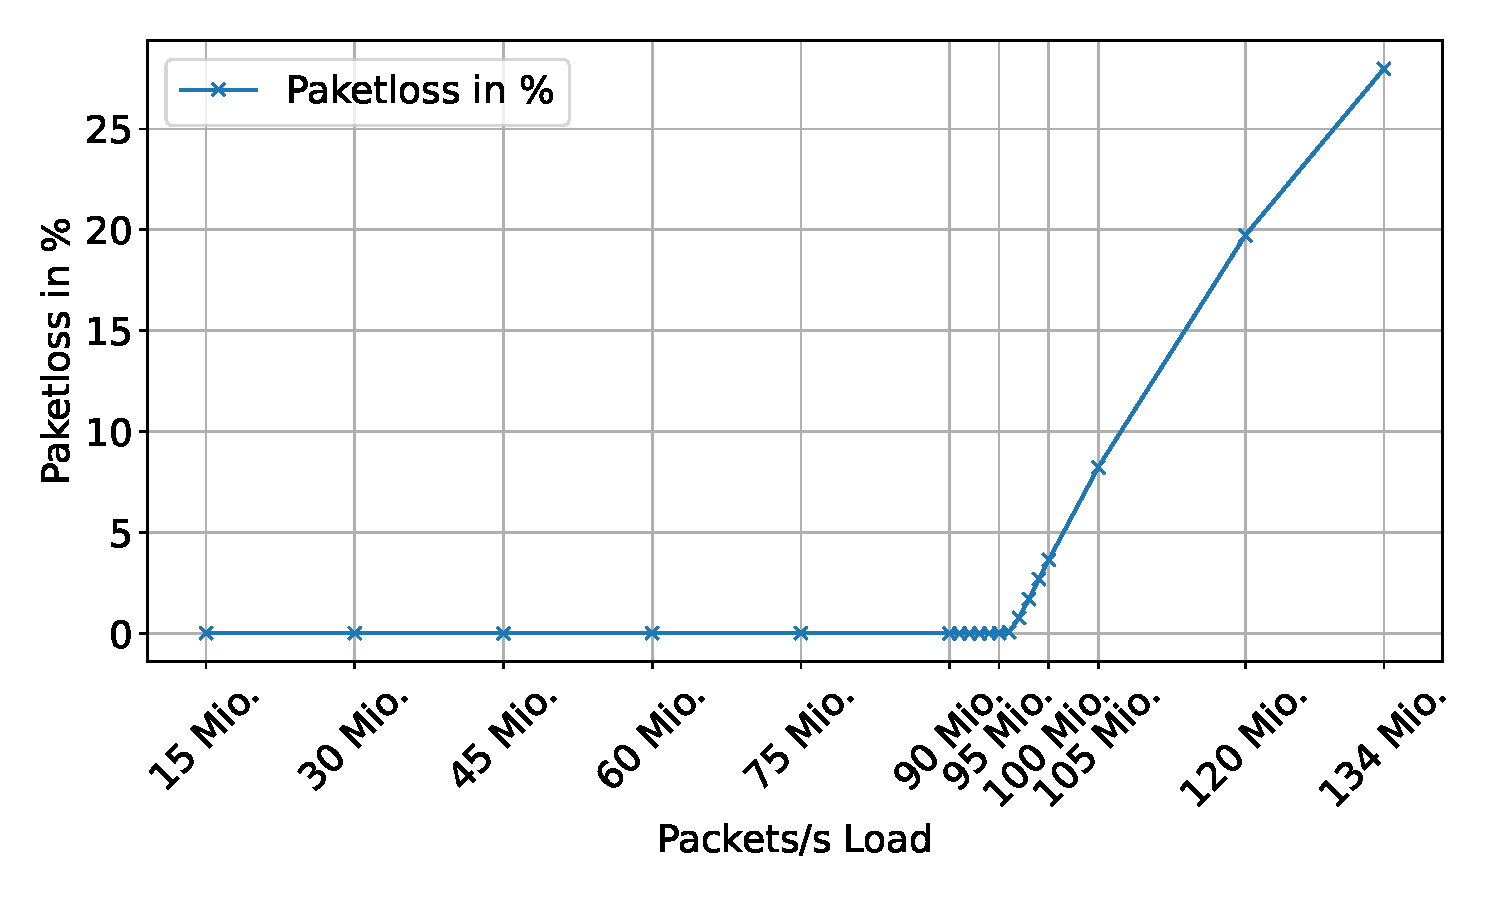
\includegraphics[width=1\linewidth]{img/pps_paketloss.pdf}
    \caption{Verlorene Pakete pro Sekunde in Prozent}
    \label{fig:placeholder}
\end{figure}
Wie in Abbildung 3.2 zu erkennen ist, war es möglich, eine Last von ca. 100 Gbit/s zu verarbeiten. Allerdings war dies nur bei einer Paketgröße von 128 Bytes möglich. Bei kleineren Paketen stellte sich als absolute Grenze der Verarbeitungsgeschwindigkeit in Paketen pro Sekunde 98 Millionen Pakete pro Sekunde bei einer Größe von weniger als 64 Byte und analog 95 Millionen Pakete pro Sekunde bei einer Größe von mehr als 64 Byte heraus. Diese abrupte Änderung ist in Abbildung 3.2 als \textit{Sudden Drop} betitelt. Wird der Schwellwert überschritten, so werden alle weiteren Pakete, wie in Abbildung 3.3 zu erkennen ist, gedroppt. Die Pakete kommen also noch auf dem Hardwareport der SmartNIC an, werden aber nicht mehr von der Verarbeitungspipeline erfasst und gehen an unbekannter Stelle verloren. Der Anstieg des entstehenden Paketloss ist fast linear, und es lässt sich somit davon ausgehen, dass das begrenzende Bottleneck die Taktung einer der verarbeitenden ASICs oder FPGAs ist. Zudem wurden Experimente zum Einfluss der Verarbeitung auf die Round-Trip-Time-Latenz durchgeführt, die gezeigt haben, dass es keinen messbaren Einfluss auf die Verarbeitungsgeschwindigkeit und Bandbreite gab. Dies war insbesondere auch unabhängig von der auf die Netzwerkkarten einwirkenden Last, da zusätzlich zu den Messpaketen auch eine künstliche Basislast erzeugt wurde, die ebenfalls auf den Loadbalancer gerichtet war.
\newpage
\section{Experimente}
\subsection{ebpf\_mac\_rewrite}
\begin{minted}{c}
SEC("xdp")
int xdp_mac_rewrite(struct xdp_md *ctx)
{
    void *data     = (void *)(long)ctx->data;
    void *data_end = (void *)(long)ctx->data_end;

    if (!bounds_ok(data, data_end, sizeof(struct ethhdr_min)))
        return XDP_ABORTED;

    struct ethhdr_min *eth = data;

    if (!bounds_ok(data, data_end, sizeof(struct ethhdr_min)))
        return XDP_ABORTED;

    struct iphdr *ip = data + sizeof(*eth);

    if ((void *)(ip + 1) > data_end)
        return XDP_DROP;

    __be32 fips1 =0x04030201;

    if ( __builtin_memcmp(&ip->saddr, &fips1, 4)) 
        return XDP_PASS;

    struct mac_addr key = {};
    __builtin_memcpy(key.addr, eth->h_source, ETH_ALEN);

    const struct mac_addr *new_dst = bpf_map_lookup_elem(&mac_redirect_map, &key);
    if (!new_dst)
        return XDP_PASS;

    __builtin_memcpy(eth->h_dest, new_dst->addr, ETH_ALEN);
    //
    // New source MAC: 63:09:DE:AD:BE:EF
    //a6:03:ff:17:2b:3a
    eth->h_source[0] = 0xA6;
    eth->h_source[1] = 0x03;
    eth->h_source[2] = 0xFF;
    eth->h_source[3] = 0x17;
    eth->h_source[4] = 0x2B;
    eth->h_source[5] = 0x3A;

    return XDP_TX;
}
\end{minted}
\subsection{max\_pipes}
\subsection{max\_entries}
\subsection{hash\_pipe}
\subsection{pcc}
\subsection{entry\_latency}
\section{Sonstiges}
\section{Fazit}
\section{Ausblick}




























\end{document}